% !TEX root = _individual/flatland.tex

%%%%%%%%%%%%%%%%%%%%%%%%%%%%%%%%%%%%%%%%%%%%%%%%%%%%%%%%%%%%%%%%%%%%%%%%%%%%%%%%
\chapter{Flatland Geometry}\label{chap:flatland}

``Flatland'' is a fictional two-dimensional universe in which particles are
constrained to exist and
travel in a 2-D plane \cite{Asa2008}. Because the flatland phase space is
$(x,y,\omega)$ with \emph{one} angular variable (the azimuthal~$\omega$),
rather than the
standard 2-D $(x,y,\mu,\omega)$ with \emph{two} angular variables (the
polar cosine~$\mu$ and the azimuthal~$\omega$),
flatland is a computationally simpler testing ground that retains the
complexity of multidimensional geometry. For this reason, flatland has recently
been used in the development and testing of multi-D transport methods, including
the new anisotropic diffusion method \cite{Lar2009c,Bor2010,Joh2011,Tra2011}.

Previous work has shown that the 3-D diffusion coefficient
$\frac{1}{3\sigma}$ differs from the flatland diffusion coefficient
$\frac{1}{2\sigma}$, but accurate boundary conditions for the flatland
diffusion equations have not been derived. An accurate diffusion
boundary condition is needed for benchmarking new transport methods, such as
anisotropic diffusion, against
diffusion solutions. Thus, in this chapter we derive ``Marshak''
and ``variational'' boundary conditions for the flatland diffusion equation.
We also present Monte Carlo sampling algorithms tailored to flatland
geometry, as well as a quick description of how 2-D \SN\ transport can easily be
adapted to flatland.

These methods are implemented in flatland primarily for the purpose of
comparison with the new anisotropic diffusion methods. We briefly derive the
AD approximation in flatland geometry for use in our benchmark problems.

%For the purposes of comparison, we also consider Fig.~\ref{fig:chordFlatland} as
%a sagittal view of an infinite cylinder; Fig.~\ref{fig:chordRz} shows a
%cross-sectional view.
%
%\begin{figure}[htb]
%  \centering
%  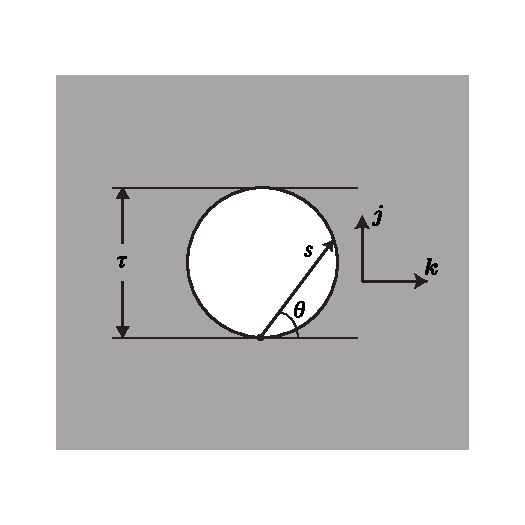
\includegraphics{chord-rz}
%  \Caption{A cross-section of the chord length problem in cylindrical
%  geometry.}{The orthogonal view looks like Fig.~\ref{fig:chordFlatland}.}
%  \label{fig:chordRz}
%\end{figure}

%%%%%%%%%%%%%%%%%%%%%%%%%%%%%%%%%%%%%%%%%%%%%%%%%%%%%%%%%%%%%%%%%%%%%%%%%%%%%%%%
\clearpage
\section{Transport}

To briefly illustrate the difference between flatland and 2-D geometry, we
view an infinite gap between two materials. The flatland problem and the
two-dimensional projection are identical, shown in Fig.~\ref{fig:chordFlatland}.
%
\begin{figure}[htb]
  \centering
  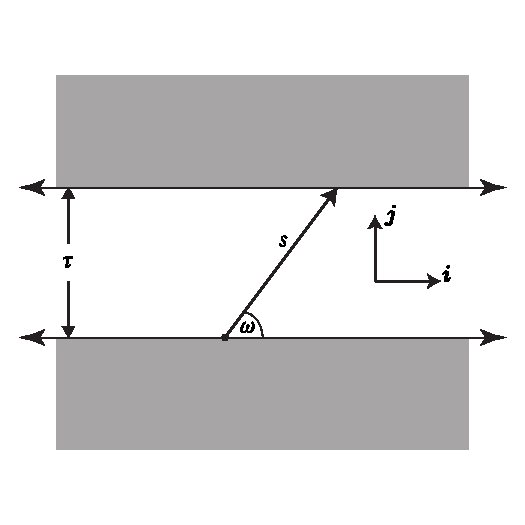
\includegraphics{chord-flatland}
  \Caption{The infinite gap as represented on paper.}%
  {The infinite gap as represented on paper. The gap is a distance
  $\tau$ across, $\omega$ is the azimuthal angle, and $s$ is the
  distance across the gap.}
  \label{fig:chordFlatland}
\end{figure}
%
However, in the 2-D case, the figure is merely a slice of a three-dimensional
problem in which the two gray rectangles and the gap are infinite in extent
(Fig.~\ref{fig:chordXy}). In the flatland case, the polar angle $\theta$ is
effectively fixed at $\theta=\pi/2$, i.e., $\mu=\cos\theta = 0$.
%
\begin{figure}[htb]
  \centering
  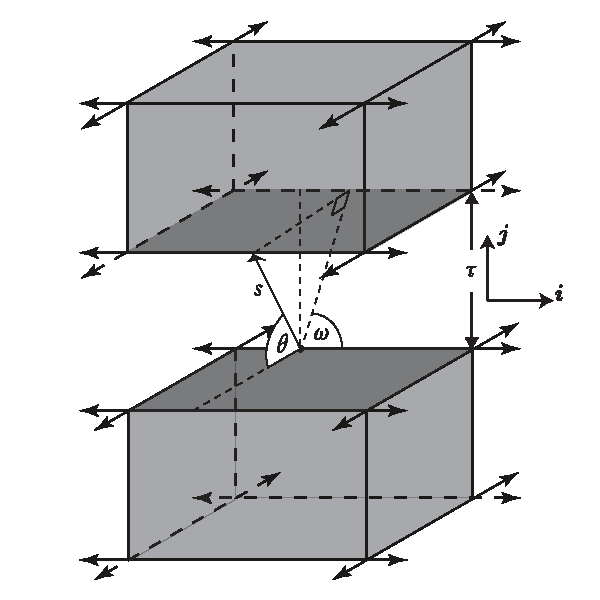
\includegraphics{chord-xyz}
  \Caption{A 3-D view of the ``2-D'' infinite gap.}{
    The polar angle cosine is $\mu= \cos \theta$, and the azimuthal angle is
  $\omega$.}
  \label{fig:chordXy}
\end{figure}

Because the time-dependent and nonlinear terms of thermal radiative transfer are
not affected by the choice of geometry, we constrain our discussion in this
section to steady-state transport. Our application of the flatland
transport equation
has only isotropic emission (and ``pseudo-scattering'' if the linearized
transport equation is used), so we limit our study to the case of isotropic
scattering.

To begin, we write the steady-state transport equation with isotropic scattering
in a ``general geometry'' form valid both for flatland and real space (1-D,
2-D, and 3-D):
\begin{subequations} \label{eqs:ssTransport}
\begin{equation}\label{eq:ssTransportVol}
  \vec{\Omega}\vd \grad I(\vec{x}, \vec{\Omega})
  + \sigma(\vec{x}) I(\vec{x}, \vec{\Omega})
  = \frac{c(\vec{x}) \sigma(\vec{x})}{\gamma_0} \phi(\vec{x})
  + \frac{1}{\gamma_0} q(\vec{x}) \,,
  \quad \vec{x} \in V \,,\ \vec{\Omega} \in S\,.
\end{equation}
Here, we use the following definitions:
\begin{align*}
  I(\vec{x},\vec{\Omega}) &= \text{the steady-state angular intensity,} \\
  \vec{\Omega} &= \text{the unit direction vector,} \\
  S &= \text{the domain of the direction vector (the ``unit sphere''),} \\
  \gamma_n &= \text{the $n$th angular moment,} \\
  c(\vec{x}) &= \text{the scattering ratio, and} \\
  \phi(\vec{x}) &= \text{the scalar intensity, i.e.~the zeroth angular moment of $I$.}
\end{align*}
The direction vectors $\vec{\Omega}$ and domains $S$ are presented in
Table~\ref{tab:angularDomain}, and the moments $\gamma_0$ are evaluated in
Table~\ref{tab:angularMoments}. The specified incident radiation
boundary:
\begin{equation} \label{eq:ssBndy}
  I(\vec{x}, \vec{\Omega}) = I^b(\vec{x}, \vec{\Omega})
  \quad \vec{x} \in \partial V \,,\ \vec{\Omega} \vd \vec{n} < 0\,.
\end{equation}
\end{subequations}

\begin{table}[htb]
  \centering
  \begin{tabular}{rccc}
\toprule
   Geometry & $\vec{\Omega}$ & Domain $S$ & $\ud\Omega$
\\ \midrule
   1-D & $\mu$ & $-1 \le \mu \le 1$ & $\ud\mu$
   \\
   2-D & $\sqrt{1-\mu^2} \cos \omega \vec{i}
   + \sqrt{1-\mu^2} \sin \omega \vec{j}$
   & $-1 \le \mu \le 1$, $0 \le \omega < 2\pi$ & $\ud\mu \ud \omega$
   \\
   Flatland & $\cos \omega \vec{i} + \sin \omega \vec{j}$
   & $0 \le \omega < 2\pi$ & $\ud \omega$
   \\
   3-D & $\mu \vec{i}
   + \sqrt{1-\mu^2} \cos \omega \vec{j}
   + \sqrt{1-\mu^2} \sin \omega \vec{k}$
   & $-1 \le \mu \le 1$, $0 \le \omega < 2\pi$ & $\ud\mu \ud \omega$
\\ \bottomrule
  \end{tabular}
  \caption{Angular variables in the various geometries.}
  \label{tab:angularDomain}
\end{table}

\begin{table}[htb]
  \centering
  \begin{tabular}{rccc}
\toprule
   Geometry
   & $\gamma_0 \equiv \int_S \ud\Omega$
   & $\gamma_1 \equiv \int_S \abs{\vec{\Omega}\vd\vec{i}} \ud\Omega$
   & $\gamma_2 \equiv \int_S (\vec{\Omega}\vd\vec{i})^2 \ud\Omega$
\\ \midrule
   1-D & 2 & 1 & $\frac{2}{3}$
   \\
   2-D & $4\pi$ & $2\pi$ & $\frac{4\pi}{3}$
   \\
   Flatland & $2\pi$ & $4$ & $\pi$
   \\
   3-D & $4\pi$ & $2\pi$ & $\frac{4\pi}{3}$
\\ \bottomrule
  \end{tabular}
  \caption{Angular moments in each geometry.}
  \label{tab:angularMoments}
\end{table}

The ``unit sphere''---%
the domain of the unit direction $\vec{\Omega}$---%
differs among the geometries. In 3-D, the direction variable is a unit vector,
$\norm{\vec{\Omega}}=1$, so valid angles
lie on the surface of a sphere of unit radius. In 2-D, those angles are
projected onto a slice through the sphere's middle, so that
$\norm{\vec{\Omega}} \le 1$: valid angles are on a unit disc. Angles on the edge
of the disc---the unit circle---represent particles traveling along the slice,
and angles inside the unit circle are the projection of 3-D angles traveling with a
non-zero polar angle cosine. Flatland geometry allows only angles on the unit
circle, $\norm{\vec{\Omega}}=1$.

%%%%%%%%%%%%%%%%%%%%%%%%%%%%%%%%%%%%%%%%
\subsection{Monte Carlo sampling}

In numerically testing the anisotropic diffusion approximation, we use Monte
Carlo methods (with a very large number of particles) to generate the reference
solutions.
The Monte Carlo method approximates the transport equation by tracking the
random histories of statistically large numbers of particles as they traverse a
problem. The behavior during their lifetime depends on probability distribution
functions (PDFs) that describe how they are born, how far they travel without a
collision, how they behave when they collide, et cetera \cite{Lew1984,Bro2004a}.

In this section, we form and discuss the probability distributions particular to
flatland geometry. We briefly derive those PDFs,
integrate them to get cumulative distribution functions
(CDFs), and use the direct inversion method to show how a uniformly sampled
pseudo-random number $\xi \in [0,1)$ may be used to determine particle behavior
in flatland. Because the geometry tracking routines of steady state Monte Carlo
and Fleck and Cummings' IMC are identical, the results in this section are
applicable to any flatland Monte Carlo implementation.

\subsubsection{Isotropic volume source}
A particle emitted from an isotropic internal source, whether an extraneous
radiation source or an indirect isotropic scattering event, has an equal
probability of entering any angle. In any geometry, the normalized PDF that
represents this process is
\begin{equation*}
  f(\vec{\Omega}) \ud\Omega = \alpha \ud\Omega \,,
  \quad \vec{\Omega} \in S \,,
\end{equation*}
where $\Omega$ is the angular domain of the
geometry (see Table~\ref{tab:angularDomain}), and $\alpha$ is a normalization
constant.
Requiring the PDF to integrate to unity over its domain gives the
following value for $\alpha$ in any geometry:
\begin{align*}
  1 = \int_{\Omega} f(\vec{\Omega}) \ud\Omega
  = \alpha \int_{\Omega} \ud\Omega = \alpha \gamma_0
  \lra
  \alpha = \frac{1}{\gamma_0}\,.
\end{align*}
Thus, the angular distribution of an isotropic volume source is
\begin{equation}\label{eq:volumeSourcePdf}
  f(\vec{\Omega}) \ud\Omega = \frac{\ud\Omega}{\gamma_0} \,,
  \quad \vec{\Omega} \in S\,.
\end{equation}

In 2-D, using the identities from Tables~\ref{tab:angularDomain}
and~\ref{tab:angularMoments}, Eq.~\eqref{eq:volumeSourcePdf} evaluates to the
familiar
\begin{equation*}
  f(\mu,\omega) \ud\mu\ud\omega = \frac{\ud\mu\ud\omega}{4\pi} 
  = \frac{\ud\mu}{2}\frac{\ud\omega}{2\pi}
  \,,
  \quad -1\le \mu \le 1,\ 0 \le \omega < 2\pi\,,
\end{equation*}
which, integrated, yields the separable CDF
\begin{equation*}
  F(\mu,\omega) = F_1(\mu) F_2(\omega)
  = \frac{1 + \mu}{2}\frac{\omega}{2\pi}\,,
  \quad -1\le \mu \le 1,\ 0 \le \omega < 2\pi\,.
\end{equation*}
Setting two uniformly sampled random numbers $\xi_1 = F_1(\mu)$ and
$\xi_2 = F_2(\omega)$, solving for $\mu$ and $\omega$, and
introducing them back into the 2-D representation of $\vec{\Omega}$, we obtain the
new direction for an isotropically emitted particle in 2-D:
\begin{align*}
  \vec{\Omega} &= \sqrt{1-\mu^2} \cos \omega \vec{i}
  + \sqrt{1-\mu^2} \sin \omega \vec{j}
\\
  &= \sqrt{1-(2\xi_1-1)^2} \cos(2\pi\xi_2) \vec{i}
  + \sqrt{1-(2\xi_1-1)^2} \sin(2\pi\xi_2) \vec{j}\,.
\end{align*}

In flatland, Eq.~\eqref{eq:volumeSourcePdf} becomes the simpler
\begin{equation*}
  f(\omega) \ud\omega = \frac{\ud\omega}{2\pi} \,,
  \quad 0 \le \omega < 2\pi\,,
\end{equation*}
yielding the CDF
\begin{equation}\label{eq:volumeSourceFlatland}
  F(\omega) = \frac{\omega}{2\pi}\,,
  \quad 0 \le \omega < 2\pi\,,
\end{equation}
Setting $\xi_1 = F(\omega)$ and solving for $\omega = F\inv(\xi_1)$ gives the
following simple relation between an isotropically sampled angle $\omega$ and a
uniformly sampled random number $\xi_1$:
\begin{equation*}
  \omega = 2\pi \xi_1\,.
\end{equation*}
The flatland particle's new angle is therefore
\begin{equation*}
  \vec{\Omega} = \cos \omega \vec{i} + \sin \omega \vec{j}
  = \cos(2\pi\xi_1) \vec{i} + \sin(2\pi\xi_1) \vec{j}\,.
\end{equation*}

With only one independent variable that needs sampling, and the omission of
the transcendental operation $\sqrt{1-\mu^2}$, the computational cost of a
scattering event is less in flatland than in 2-D, leading to
faster simulation times.

\subsubsection{Isotropic surface source}\label{sec:isoSurface}
Particles emitted from an isotropic surface source have a cosine distribution
\cite{Gre2002}, in which the partial first moment in each differential angle is
constant. The PDF for a surface source is
\begin{equation*}
  f(\vec{\Omega}) \ud\Omega = \alpha \abs{\vec{\Omega}\vd \vec{n}} \ud\Omega \,,
\quad \vec{\Omega}\vd \vec{n} < 0 \,,
\end{equation*}
where $\alpha$ is a normalization constant. We obtain $\alpha$ by integrating over
the angular domain and substituting the angular moments from Table~\ref{tab:angularMoments}:
\begin{align*}
  1 &= \int_{\vec{\Omega}\vd \vec{n} < 0} \left[ \alpha \abs{\vec{\Omega}\vd
  \vec{n}} \right] \ud\Omega
  \\
  1 &=\frac{\alpha}{2} \int_{\Omega} \abs{\vec{\Omega}\vd \vec{n}} \ud\Omega
  \\
  \alpha &= \frac{2}{\gamma_1}\,.
\end{align*}
Thus, the normalized PDF for an isotropic surface source is
\begin{equation}\label{eq:surfaceSourcePdf}
  f(\vec{\Omega}) \ud\Omega = \frac{2}{\gamma_1} \abs{\vec{\Omega}\vd \vec{n}} \ud\Omega \,,
\quad \vec{\Omega}\vd \vec{n} < 0 \,.
\end{equation}

In 3-D, choosing $\vec{n}=\vec{i}$, the isotropic surface PDF is
\begin{equation*}
  f(\mu,\omega) \ud\mu \ud\omega
  = \frac{1}{\pi} \mu \ud\mu \ud\omega
  = (2 \mu \ud\mu) \frac{\ud\omega}{2\pi}\,,
\end{equation*}
which gives the separable CDF
\begin{equation*}
  F(\mu,\omega) = \mu^2 \frac{\omega}{2\pi}\,.
\end{equation*}
The sampled directions are thus $\mu=\sqrt{\xi_1}$ and $\omega=2\pi \xi_2$.

In flatland, the surface source distribution is different. Let us choose
$\vec{n} = -\vec{j}$ so that emitted particles have azimuthal angles in the range
$\omega \in [0, \pi)$.
Applying the flatland identities in Tables~\ref{tab:angularDomain}
and~\ref{tab:angularMoments} to Eq.~\eqref{eq:surfaceSourcePdf}, we obtain
the following surface source PDF for flatland:
\begin{equation*}
  f(\omega) \ud\omega = \frac{2}{4} \, \abs{ -\sin \omega}\ud\omega
  = \frac{1}{2} \sin \omega\ud\omega \,,\quad 0 \le \omega < \pi\,.
\end{equation*}
The corresponding CDF is
\begin{equation}\label{eq:surfaceSourceFlatland}
  F(\omega) = \frac{1}{2} \left( 1-\cos\omega \right)
  \,,\quad 0 \le \omega < \pi\,.
\end{equation}
Solving for $\omega = F\inv(\xi_1)$ gives the sampled azimuthal angle for a surface source
in flatland:
\begin{equation*}
  \omega = \cos\inv(1 - 2\xi_1)\,.
\end{equation*}
Finally, we insert this sampled angle into the flatland
direction vector $\vec{\Omega}$ and use the identity
$\cos^2 \omega + \sin^2 \omega = 1$ to reduce the number of transcendental
functions. Thus the sampled direction of a particle from an isotropic surface
source is:
\begin{align*}
  \vec{\Omega} &= \cos \omega \vec{i} + \sin \omega \vec{j} \\
  &=  \cos[ \cos\inv(1 - 2\xi_1) ] \vec{i} + \sin[ \cos\inv(1 - 2\xi_1) ] \vec{j} \\
  &= (1 - 2\xi_1) \vec{i} + \sqrt{1 - (1 - 2\xi_1)^2} \vec{j}\,.
\end{align*}

%%%%%%%%%%%%%%%%%%%%%%%%%%%%%%%%%%%%%%%%
\subsection{Discrete ordinates quadrature}\label{sec:flatlandQuadrature}

A standard practice in two-dimensional discrete ordinates (\SN) solvers is to
create a quadrature set with polar angles that encompass only the top half of a
unit sphere, $\mu>0$, and to modify the ordinate weights so that they sum to
$4\pi$
\cite{Zik1997}. Well-constructed quadrature sets will also correctly
integrate the spherical harmonic functions \cite{Rab2007} over the unit sphere.
The odd spherical harmonic functions will automatically integrate to zero, and
the even
functions are linear combinations of the even angular moments of
Table~\ref{tab:angularMoments}:
\begin{equation*}
  \gamma_n
  = \sum_{m=1}^{M} \abs{ \vec{\Omega}_m \vd \vec{i}}^n w_m
  = \int_S \abs{ \vec{\Omega}\vd\vec{i} }^n \ud\Omega \,,\ n\ \text{even}.
\end{equation*}
Most quadrature sets do not exactly integrate partial odd moments.

The most straightforward way to implement a \emph{flatland} \SN\
code with only isotropic scattering is to use an existing 2-D \SN\ code with a
special quadrature set
consisting of ordinates that have a single
polar angle $\mu=0$. Using a Chebyshev--Gauss quadrature of the first kind
\cite{Str1966a} for the azimuthal angles will preserve the flatland angular moments,
\begin{equation*}
  \gamma_n
  = \sum_{m=1}^{M} \sin^n \theta_m w_m
  = \int_{2\pi} \sin^n \theta \ud\theta\,,\ n\ \text{even} \,.
\end{equation*}
A quadrature set with $2M$ total ordinates (i.e., $M$ per two octants, the
standard nomenclature for discrete ordinates quadratures) will exactly integrate
the first $2M-1$ polynomials of $x=\sin \theta$. The procedure to calculate
a Chebyshev quadrature set for the first quadrant is:
\begin{enumerate}
  \item Solve for the roots of an $2M$-order Chebyshev polynomial of the first
    kind on $[-1,1]$. Discard the negative roots.
  \item Take the inverse sine of the positive roots. These $M$ roots are the
    ordinate directions $\theta_m$ in the first quadrant.
  \item Assign the uniform weight $w_m = \frac{\pi}{M}$.
\end{enumerate}
For ease of implementation, we normalized the quadrature weights so that they sum
to $4\pi$ instead of $2\pi$. This allows flatland quadrature sets to be used in
an existing 2-D discrete ordinates code in which the scattering kernel expects the
quadrature set to be normalized to $4\pi$. Table~\ref{tab:chebyQs} gives several
orders of the Chebyshev quadrature set with sixteen digits of precision; a more
extensive and computer-readable set of ordinates is available online at
\url{https://github.com/sethrj/PyTRT/blob/master/tools/python/qs/cgvalues2.json}.

\begin{table}[p]
  \centering\small%
\begin{minipage}[t]{3in}
\null% needed to align tops
\hspace{\stretch{1}}
\begin{tabular}{l@{}l} \toprule
\multicolumn{2}{c}{$N=2$, $w=\pi$ } \\ \midrule
$\omega_{0}$ & ${}=0.7853981633974483$ \\ \toprule
\multicolumn{2}{c}{$N=4$, $w=\pi / 2$ } \\ \midrule
$\omega_{0}$ & ${}=0.3926990816987241$ \\
$\omega_{1}$ & ${}=1.1780972450961724$ \\ \toprule
\multicolumn{2}{c}{$N=8$, $w=\pi / 4$ } \\ \midrule
$\omega_{0}$ & ${}=0.1963495408493621$ \\
$\omega_{1}$ & ${}=0.5890486225480862$ \\
$\omega_{2}$ & ${}=0.9817477042468103$ \\
$\omega_{3}$ & ${}=1.3744467859455345$ \\ \toprule
\multicolumn{2}{c}{$N=16$, $w=\pi / 8$ } \\ \midrule
$\omega_{0}$ & ${}=0.0981747704246810$ \\
$\omega_{1}$ & ${}=0.2945243112740431$ \\
$\omega_{2}$ & ${}=0.4908738521234052$ \\
$\omega_{3}$ & ${}=0.6872233929727672$ \\
$\omega_{4}$ & ${}=0.8835729338221293$ \\
$\omega_{5}$ & ${}=1.0799224746714915$ \\
$\omega_{6}$ & ${}=1.2762720155208536$ \\
$\omega_{7}$ & ${}=1.4726215563702156$ \\ \toprule
\multicolumn{2}{c}{$N=32$, $w=\pi / 16$ } \\ \midrule
$\omega_{0}$ & ${}=0.0490873852123405$ \\
$\omega_{1}$ & ${}=0.1472621556370216$ \\
$\omega_{2}$ & ${}=0.2454369260617026$ \\
$\omega_{3}$ & ${}=0.3436116964863836$ \\
$\omega_{4}$ & ${}=0.4417864669110647$ \\
$\omega_{5}$ & ${}=0.5399612373357457$ \\
$\omega_{6}$ & ${}=0.6381360077604268$ \\
$\omega_{7}$ & ${}=0.7363107781851078$ \\
$\omega_{8}$ & ${}=0.8344855486097889$ \\
$\omega_{9}$ & ${}=0.9326603190344699$ \\
$\omega_{10}$ & ${}=1.0308350894591509$ \\
$\omega_{11}$ & ${}=1.1290098598838318$ \\
$\omega_{12}$ & ${}=1.2271846303085130$ \\
$\omega_{13}$ & ${}=1.3253594007331939$ \\
$\omega_{14}$ & ${}=1.4235341711578751$ \\
$\omega_{15}$ & ${}=1.5217089415825562$ \\
\bottomrule
\end{tabular}%
\hspace{\stretch{1}}
\end{minipage}%
%
\begin{minipage}[t]{3in}
\null% needed to align tops
\hspace{\stretch{1}}
\begin{tabular}{l@{}l} \toprule
\multicolumn{2}{c}{$N=64$, $w=\pi / 32$ } \\ \midrule
$\omega_{0}$ & ${}=0.0245436926061703$ \\
$\omega_{1}$ & ${}=0.0736310778185108$ \\
$\omega_{2}$ & ${}=0.1227184630308513$ \\
$\omega_{3}$ & ${}=0.1718058482431918$ \\
$\omega_{4}$ & ${}=0.2208932334555323$ \\
$\omega_{5}$ & ${}=0.2699806186678729$ \\
$\omega_{6}$ & ${}=0.3190680038802134$ \\
$\omega_{7}$ & ${}=0.3681553890925539$ \\
$\omega_{8}$ & ${}=0.4172427743048944$ \\
$\omega_{9}$ & ${}=0.4663301595172349$ \\
$\omega_{10}$ & ${}=0.5154175447295755$ \\
$\omega_{11}$ & ${}=0.5645049299419159$ \\
$\omega_{12}$ & ${}=0.6135923151542565$ \\
$\omega_{13}$ & ${}=0.6626797003665970$ \\
$\omega_{14}$ & ${}=0.7117670855789375$ \\
$\omega_{15}$ & ${}=0.7608544707912781$ \\
$\omega_{16}$ & ${}=0.8099418560036186$ \\
$\omega_{17}$ & ${}=0.8590292412159591$ \\
$\omega_{18}$ & ${}=0.9081166264282996$ \\
$\omega_{19}$ & ${}=0.9572040116406402$ \\
$\omega_{20}$ & ${}=1.0062913968529807$ \\
$\omega_{21}$ & ${}=1.0553787820653211$ \\
$\omega_{22}$ & ${}=1.1044661672776617$ \\
$\omega_{23}$ & ${}=1.1535535524900022$ \\
$\omega_{24}$ & ${}=1.2026409377023428$ \\
$\omega_{25}$ & ${}=1.2517283229146832$ \\
$\omega_{26}$ & ${}=1.3008157081270237$ \\
$\omega_{27}$ & ${}=1.3499030933393643$ \\
$\omega_{28}$ & ${}=1.3989904785517049$ \\
$\omega_{29}$ & ${}=1.4480778637640452$ \\
$\omega_{30}$ & ${}=1.4971652489763858$ \\
$\omega_{31}$ & ${}=1.5462526341887264$ \\
\bottomrule
\end{tabular}%
\hspace{\stretch{1}}
\end{minipage}%
\Caption{Chebyshev--Gauss flatland quadrature sets.}{
  Orders 2, 4, 8, 16, 32, and 64 are given for the
  first quadrant. The weights in each order are equal and sum to $4\pi$.}
  \label{tab:chebyQs}
\end{table}

In order to demonstrate the effect of this weight renormalization, let us
consider the calculation of the anisotropic diffusion tensor
in a homogeneous medium.  The purely absorbing flatland transport problem has the
solution $f(\vec{\Omega}) = \frac{1}{2\pi\sigma}$, which yields the diffusion
coefficient
\begin{equation*}
  \Dtens = \int_{0}^{2\pi} \vec{\Omega}\vec{\Omega} f(\vec{\Omega}) \ud \omega
  = \frac{1}{2\sigma} \Identitytens \,.
\end{equation*}
In an \SN\ calculation implemented with modified quadrature weights, the
transport solution for each angle $m$ will yield $f_m = \frac{1}{4\pi\sigma}$,
and the quadrature integration will yield
\begin{equation*}
  \Dtens = \sum_{m=1}^{M} \vec{\Omega}_m \vec{\Omega}_m f_m  w_m 
  = \frac{1}{2\sigma} \Identitytens \,.
\end{equation*}
This implementation therefore will calculate correct low-order angular moments of
the transport solution, but the apparent value of each $f_m$ is one half 
the correct value. Thus, for example, visualizing the \SN\
solution by plotting $f_m$ as a function of $\omega_m$ requires multiplying by a
factor of two.

%%%%%%%%%%%%%%%%%%%%%%%%%%%%%%%%%%%%%%%%%%%%%%%%%%%%%%%%%%%%%%%%%%%%%%%%%%%%%%%%
\section{Diffusion}

An accurate flatland diffusion formulation
is needed for benchmarking the anisotropic diffusion
approximation against diffusion solutions.
In the following section we derive ``Marshak'' and ``variational'' boundary
conditions for the flatland diffusion equation. (A summary of this original
work is published in Ref.~\cite{Joh2011a}.)
%There is no loss of generality in
%ignoring the time dependence because of the quasi-static approximation made in
%the derivation of the diffusion coefficient (see \S\ref{sec:bgDiffusion}).

The difference between diffusion in flatland and 2-D results from the
angular moments in the two geometries, which
are defined (and evaluated in Table~\ref{tab:angularMoments}) as:
\begin{equation*}
  \gamma_n \equiv \int_S \abs{\vec{\Omega} \vd \vec{i}}^n \ud\Omega\,.
\end{equation*}
These give rise not only to a different diffusion coefficient in the interior
but also different boundary conditions.

%%%%%%%%%%%%%%%%%%%%%%%%%%%%%%%%%%%%%%%%
\subsection{Interior diffusion approximation}

The diffusion approximation begins by assuming that $I$ is linear in angle:
\begin{equation*}
  I(\vec{x}, \vec{\Omega}) \approx f(\vec{x}) + \vec{\Omega} \vd
  \vec{g}(\vec{x})\,.
\end{equation*}
The zeroth angular moment of $I$ determines $f$:
\begin{equation*}
  \phi = \int_S I \ud\Omega
= \int_S \left( f + \vec{\Omega}\vd \vec{g} \right) \ud\Omega
= \int_S\ud\Omega f + 0
= \gamma_0 f \,,
\end{equation*}
and the first moment of $I$ determines $g$:
\begin{equation*}
  \vec{F} = \int_S \vec{\Omega} I \ud\Omega
= f \int_S \vec{\Omega} \ud\Omega
  + \vec{g} \vd \int_S \vec{\Omega}\vec{\Omega} \ud\Omega
= \gamma_2 \vec{g} \,.
\end{equation*}
This is the \Pone\ approximation to the radiation intensity:
\begin{equation}\label{eq:ssPone}
  I(\vec{x}, \vec{\Omega})
  \approx \frac{1}{\gamma_0} \phi(\vec{x})
  + \frac{1}{\gamma_2} \vec{\Omega} \vd \vec{F}(\vec{x})\,.
\end{equation}

The diffusion approximation is a closure for the first angular moment of
the transport equation. Operating on Eq.~\eqref{eq:ssTransportVol} by
$\int_S \vec{\Omega} (\cdot) \ud\Omega$ and substituting
the approximation in Eq.~\eqref{eq:ssPone} reduces the first angular moment of
the transport equation to the following:
\begin{align*}
  \grad \vd \int_S \vec{\Omega} \vec{\Omega} I
  \ud\Omega
  + \sigma \int_S \vec{\Omega} I \ud\Omega
  &=
  \frac{c\sigma}{\gamma_0} \phi \int_S \vec{\Omega} \ud\Omega
  + \frac{1}{\gamma_0} q \int_S \vec{\Omega} \ud\Omega
  \\
  \grad \vd \int_S \vec{\Omega} \vec{\Omega} \left(
  \frac{1}{\gamma_0}\phi + \frac{1}{\gamma_2} \vec{\Omega} \vd \vec{F}
  \right)
  \ud\Omega
  + \sigma \vec{F}
  &= 0
  \\
  \frac{1}{\gamma_0} \grad \vd \int_S \vec{\Omega} \vec{\Omega}
  \ud\Omega\, \phi 
  + \sigma \vec{F} &= 0
  \\
  \frac{\gamma_2}{\gamma_0} \grad \phi + \sigma \vec{F} &= 0 \,.
\end{align*}
Solving for $\vec{F}$ gives Fick's law, expressed in the general form:
\begin{equation} \label{eq:fickGeneral}
  \vec{F}(\vec{x})
  = - \frac{\gamma_2}{\gamma_0} \frac{1}{\sigma(\vec{x})} \grad \phi(\vec{x})
  \equiv -D(\vec{x}) \grad \phi(\vec{x})\,.
\end{equation}
In 2-D and 3-D, $\gamma_2/\gamma_0 = (4\pi / 3) / (4\pi) = 1/3$; in
flatland, $\gamma_2/\gamma_0 = \pi / (2\pi) = 1/2$. Thus, $D=\frac{1}{3\sigma}$ in
2-D but $D=\frac{1}{2\sigma}$ in flatland.

Substituting Fick's law into the linear-in-angle approximation,
Eq.~\eqref{eq:ssPone}, we obtain the diffusion approximation to the angular
intensity:
\begin{align} \nonumber
  I(\vec{x}, \vec{\Omega})
  &\approx \frac{1}{\gamma_0} \phi(\vec{x})
  + \frac{1}{\gamma_2} \vec{\Omega} \vd \left[ - \frac{\gamma_2}{\gamma_0}
  \frac{1}{\sigma(\vec{x})} \grad \phi(\vec{x}) \right]
  \\ \label{eq:diffusionIntensity}
  I(\vec{x}, \vec{\Omega})
  &= \frac{1}{\gamma_0} \left[ \phi(\vec{x})
  - \frac{1}{\sigma(\vec{x})}
  \vec{\Omega} \vd \grad \phi(\vec{x}) \right] \,.
\end{align}
In physical geometry this is the standard diffusion approximation
\begin{equation*}
 I(\vec{x}, \vec{\Omega})
= \frac{1}{4\pi} \left[ \phi(\vec{x}) - \frac{1}{\sigma(\vec{x})} \vec{\Omega}
\vd \grad \phi(\vec{x}) \right] \,,
\end{equation*}
and in flatland, the diffusion approximation is
\begin{equation}\label{eq:flatlandDiffusion}
 I(\vec{x}, \vec{\Omega})
= \frac{1}{2\pi} \left[ \phi(\vec{x}) - \frac{1}{\sigma(\vec{x})} \vec{\Omega}
\vd \grad \phi(\vec{x}) \right]\,.
\end{equation}

%%%%%%%%%%%%%%%%%%%%%%%%%%%%%%%%%%%%%%%%
\subsection{Marshak boundary condition}
The Marshak boundary condition \cite{Mar1947} preserves the incident radiation
flux (the partial first moment for incoming directions) on the boundary. It is
derived by substituting the approximate diffusion
intensity from Eq.~\eqref{eq:diffusionIntensity} into the boundary condition,
Eq.~\eqref{eq:ssBndy}, multiplying by $\abs{\vec{\Omega}\vd \vec{n}}$, and integrating over
incident directions:
\begin{align*}
\int_{\vec{\Omega}\vd \vec{n} < 0 } \abs{\vec{\Omega}\vd \vec{n}}
I^b \ud\Omega
 &= 
\int_{\vec{\Omega}\vd \vec{n} < 0 } \abs{\vec{\Omega}\vd \vec{n}} 
 \frac{1}{\gamma_0} \left[ \phi - \frac{1}{\sigma}
  \vec{\Omega} \vd \grad \phi \right]
  \ud\Omega
\\
F^{-}
&= 
\frac{1}{\gamma_0} \phi \left( \int_{\vec{\Omega}\vd \vec{n} < 0 }
\abs{\vec{\Omega}\vd \vec{n}} \ud\Omega \right) 
  - \frac{1}{\gamma_0}\frac{1}{\sigma}
  \left( \int_{\vec{\Omega}\vd \vec{n} < 0 } [-\vec{\Omega}\vd \vec{n}]
  \vec{\Omega} \ud\Omega  \right) \vd \grad \phi
\\
F^{-}
&=
\frac{1}{\gamma_0} \phi \left( \frac{\gamma_1}{2} \right) 
  + \frac{1}{\gamma_0}\frac{1}{\sigma} \left( \vec{n} \vd
  \frac{\gamma_2}{2} \Identitytens \right)
  \vd \grad \phi
\\
F^{-}
&=
\frac{\gamma_1}{2\gamma_0} \phi
+ \frac{\gamma_2}{2\gamma_0}\frac{1}{\sigma} \vec{n} \vd \grad \phi\,.
\end{align*}
This is the Marshak diffusion boundary condition:
\begin{equation} \label{eq:marshak}
\frac{2\gamma_0}{\gamma_1} F^{-}
=
\phi + \frac{\gamma_2}{\gamma_1}\frac{1}{\sigma} \vec{n} \vd \grad \phi\,.
\end{equation}

The value
\begin{equation*}
  \frac{\gamma_2}{\gamma_1}
  =
  \begin{cases}
    \frac{2}{3} \approx 0.6667 & \text{in 1-D, 2-D, 3-D; and} \\
    \frac{\pi}{4} \approx 0.7854 & \text{in flatland,}
  \end{cases}
\end{equation*}
is the Marshak extrapolation distance.
The physical reason for the longer extrapolation distance in flatland
is that in 2-D, a greater fraction of particles travel at a steep angle to the
$x,y$-plane, yielding a steeper slope for $\phi$ on the boundary.

We can also rewrite the Marshak boundary condition in terms of the diffusion
coefficient by substituting $D$ from Eq.~\eqref{eq:fickGeneral}:
\begin{equation*}
\frac{2\gamma_0}{\gamma_1} F^{-}
= \phi + \frac{\gamma_0}{\gamma_1} D \vec{n} \vd \grad \phi\,.
\end{equation*}
In 1-D, 2-D, and 3-D geometries, this is the standard Marshak boundary condition
\begin{equation*}
4 F^{-}
= \phi + 2 D \vec{n} \vd \grad \phi\,.
\end{equation*}
In flatland, it is the following:
\begin{equation}\label{eq:flatMarshak}
\pi F^{-}
= \phi + \frac{\pi}{2} D \vec{n} \vd \grad \phi\,.
\end{equation}

%%%%%%%%%%%%%%%%%%%%%%%%%%%%%%%%%%%%%%%%
\subsection{Variational boundary condition} \label{sec:varBndy}
The Marshak boundary condition is heuristic: it attempts only to conserve the
rate of energy entering through the boundary.
A more accurate boundary condition recognizes that the diffusion
approximation is an asymptotic limit of the transport equation and uses an
asymptotic matched boundary layer analysis to relate the transport solution
on the boundary to the diffusive solution in the interior. However, a simpler
(than asymptotic) method of deriving a more accurate (than Marshak) boundary
condition is to use
a variational analysis \cite{Mal1991}.
A shorter but equivalent analysis, adapted to flatland geometry, follows.

We consider a homogeneous, source-free ($q=0$), purely scattering ($c=1$)
transport problem in a
semi-infinite flatland plane.\footnote{%
The justification for setting $c=1$ and $q=0$ relates to the asymptotic
scaling used to derive diffusion from the transport equation:
both $q$ and $1-c$ are $O(\epsilon^2)$ quantities \cite{Mal1991}.}
The transport equation~\eqref{eq:ssTransportVol} becomes
\begin{subequations} \label{eqs:flatTransport}
\begin{equation}\label{eq:flatTransportVol}
  \cos \omega \pder{I}{x} + \sin \omega \pder{I}{y} + \sigma I
  = \frac{\sigma}{2\pi} \int_{0}^{2\pi} I \ud \omega'\,,\quad
 -\infty < x < \infty,\ 0 \le y < \infty,\ 0 \le \omega < 2\pi\,.
\end{equation}
It has a uniform incident boundary condition,
\begin{equation}\label{eq:flatTransportBndy}
  I(x, 0, \omega) = I^b(\omega) \,,\quad -\infty < x < \infty,\ 
  0 \le \omega < \pi \,.
\end{equation}
\end{subequations}
%The justification for using a purely scattering problem is related to the
%asymptotic analysis that shows the transport solution to satisfy a diffusion
%equation in the ``diffusive'' limit. In this limit, absorption is scaled as
%$O(\epsilon^2)$; the full variational analysis \cite{Mal1991} yields a
%variational estimate of the transport solution also accurate to $O(\epsilon^2)$.

Because neither the boundary condition nor $\sigma$ varies
in $x$, $\tpder{I}{x}=0$, and Eq.~\eqref{eq:flatTransportVol} reduces to a
one-dimensional flatland transport equation:
\begin{equation}\label{eq:scatteringOnedFlatland}
  \sin \omega \pder{}{y}I(y,\omega) + \sigma I(y,\omega)
  = \frac{\sigma}{2\pi} \int_{0}^{2\pi} I(y,\omega') \ud \omega'\,.
\end{equation}
This is \emph{not} the 1-D planar geometry transport equation.

We define the $y$ components of the angular moments of $I$ as
\begin{equation} \label{eq:flatPhi}
  \phi_m(y) = \int_{0}^{2\pi} (\vec{\Omega}\vd\vec{j})^m I(y,\omega) \ud\omega
  = \int_{0}^{2\pi} (\sin\omega)^m I(y,\omega) \ud\omega \,.
\end{equation}
As $y\to\infty$, the intensity $I$ approaches a constant $\varphi/2\pi$,
which gives $\phi_0(\infty)=\phi(\infty)\equiv\varphi$.
Concordantly, $\phi_1(\infty)=0$.

Operating on the transport equation by $\int_{0}^{2\pi} (\sin\omega)^m (\cdot)
\ud\omega$ gives the $m$th angular moment in the $y$ direction:
\begin{align} \nonumber
  \pder{}{y} \int_{0}^{2\pi} (\sin\omega)^{m+1} I \ud\omega
  + \sigma \int_{0}^{2\pi} (\sin\omega)^{m} I \ud\omega
  &= \frac{\sigma}{2\pi} \int_{0}^{2\pi} I \ud \omega'
  \int_{0}^{2\pi} (\sin\omega)^{m} \ud\omega
  \\ \label{eq:flatMoments}
  \pder{\phi_{m+1}}{y}
  + \sigma \phi_{m}
  &= \frac{\sigma}{2\pi} \phi_{0}
  \int_{0}^{2\pi} (\sin\omega)^{m} \ud\omega\,.
\end{align}
For $m=0$, the conservation equation, Eq.~\eqref{eq:flatMoments} evaluates to
\begin{equation*}
  \pder{\phi_{1}}{y}
  + \sigma \phi_{0}
  = \frac{\sigma}{2\pi} \phi_{0} (2\pi)
  \lra
  \pder{\phi_{1}}{y} = 0\,.
\end{equation*}
Thus, the radiation flux is a constant, and because $\phi_1(\infty)=0$,
that constant is zero. Physically, $\phi_1=0$ means that at every
point, the rate of energy being transferred away from the boundary is balanced
by energy moving toward the boundary. This logically follows from the lack of
absorption in the problem: at steady-state, the only means of energy loss is
through exiting the boundary.

Evaluating Eq.~\eqref{eq:flatMoments} for $m=1$ and using the result that
$\phi_{1}=0$, we obtain
\begin{equation*}
  \pder{\phi_{2}}{y}
  + \sigma \phi_{1}
  = \frac{\sigma}{2\pi} \phi_{0} (0)
  \lra
  \pder{\phi_{2}}{y} = 0\,.
\end{equation*}
Thus $\phi_{2}$ is also a constant. At large distances from the boundary,
$y\to\infty$, the radiation assumes an isotropic distribution,
$I\to\varphi/2\pi$. From these two facts we relate the second angular moment
throughout the problem to the equilibrium scalar intensity $\varphi$:
\begin{equation*}
  \phi_{2} = \int_{0}^{2\pi} (\sin\omega)^2 \frac{\varphi}{2\pi} \ud\omega
  = \frac{1}{2} \varphi\,.
\end{equation*}
% in 1-D, this would be $\int_{-1}^{1}\mu^2\frac{\varphi}{2} \ud \mu =
% \frac{1}{3} \varphi$.

Since $\phi_1=0$, we can add $\alpha \phi_1$ to the previous equation for any
$\alpha$:
\begin{align*}
 \alpha\phi_1 + \phi_{2} &= \frac{\varphi}{2} \\
 \int_{0}^{2\pi} (\alpha \sin\omega + \sin^2\omega)
 I(y,\omega) \ud\omega
 &= \frac{\varphi}{2}\,.
\end{align*}
At the boundary $y=0$, $I=I^b$ for incident angles $0 \le \omega < \pi$.
The variational analysis in Ref.~\cite{Mal1991} reveals that certain trial functions
allow an exiting angular distribution that is isotropic to second order accuracy,
so we make the ``variational'' approximation that $I(0,\omega)=I^\text{out}$.
The previous equation then yields
\begin{equation*}
 \int_{0}^{\pi} (\alpha \sin\omega + \sin^2\omega)
 I^b(\omega) \ud\omega
 + \int_{\pi}^{2\pi} (\alpha \sin\omega + \sin^2\omega)\ud\omega I^\text{out}
 = \frac{\varphi}{2}\,.
\end{equation*}
The value $\alpha=\pi/4$ eliminates the integral over outgoing directions and
gives the following relation between moments of the incident angular flux and the
magnitude of the angular flux as $y\to\infty$:
\begin{equation}\label{eq:varBoundary}
 \varphi = 2\int_{0}^{\pi} \left( \frac{\pi}{4} \sin\omega + \sin^2\omega \right)
 I^b(\omega) \ud\omega
 \,.
\end{equation}

We wish our boundary condition to preserve the value of
$\varphi$ when the diffusion method is used, so we substitute the diffusion
approximation, Eq.~\eqref{eq:flatlandDiffusion}:
\begin{align*}
 \varphi &= 2\int_{0}^{\pi} \left( \frac{\pi}{4} \sin\omega + \sin^2\omega \right)
 I^b(\omega) \ud\omega
 \\
 &= 
  2\int_{0}^{\pi} \left( \frac{\pi}{4} \sin\omega + \sin^2\omega \right)
 \left( \frac{1}{2\pi} \phi -
  \frac{1}{\sigma} \sin\omega \pder{\phi}{y}\right)\ud\omega
\\
 &= 
\frac{1}{2\pi} \int_{0}^{\pi} \left( \frac{\pi}{2} \sin\omega + 2 \sin^2\omega
\right)\ud\omega
 \,\phi -
 \frac{1}{2\pi} \int_{0}^{\pi} \left( \frac{\pi}{2} \sin^2\omega + 2 \sin^3\omega \right)\ud\omega
  \,\frac{1}{\sigma} \pder{\phi}{y}
  \\
 &= 
 \frac{1}{2\pi} \left( \frac{\pi}{2} [2] + 2 \frac{\pi}{2}
\right) \phi
-
\frac{1}{2\pi} \left( \frac{\pi}{2} \left[ \frac{\pi}{2} \right] + 2 \left[
\frac{4}{3} \right] \right) \frac{1}{\sigma} \pder{\phi}{y}
\\
 &= 
  \phi
- \left( \frac{\pi}{8} + \frac{4}{3\pi} \right) \frac{1}{\sigma} \pder{\phi}{y}
\,.
\end{align*}
In this problem, the boundary surface outer normal is $\vec{n}=-\vec{j}$. 
Replacing $\sin \omega$ with $-\vec{\Omega}\vd\vec{n}$, we obtain the following
flatland variational boundary condition:
\begin{equation} \label{eq:flatVarBc}
\int_{\vec{\Omega}\vd\vec{n} < 0} \left[ \frac{\pi}{2}
\abs{\vec{\Omega}\vd\vec{n}} + 2 (\vec{\Omega}\vd\vec{n})^2 \right]
I^b(\vec{x}, \vec{\Omega}) \ud\Omega
= 
  \phi(\vec{x})
  - \left( \frac{\pi}{8} + \frac{4}{3\pi} \right) \frac{1}{\sigma}
  \vec{n}\vd\grad \phi(\vec{x})\,.
\end{equation}
Compared to the flatland Marshak boundary condition,
Eq.~\eqref{eq:flatMarshak}, the variational boundary condition not only yields a
different extrapolation distance $\frac{\pi}{8} + \frac{4}{3\pi} \approx
0.8171$ but also uses a different moment of the incident boundary flux.

%%%%%%%%%%%%%%%%%%%%%%%%%%%%%%%%%%%%%%%%
\subsection{Generalization}\label{sec:flatlandV}

We recall from the discussion of boundary conditions in
Chapter~\ref{chap:adDerivation} that to eliminate the boundary layer solution
in the interior of a 3-D problem, the necessary condition is
\begin{equation}\label{eq:tdKillBndy_6}
  \int_{\vec{\Omega}\vd\vec{n} < 0}
  W(\abs{\vec{\Omega}\vd\vec{n}}) \Ibl(\vec{x},\vec{\Omega}) \ud\Omega
  = 0\,,
  \quad \vec{x}\in \partial V ,\ \vec{\Omega}\vd \vec{n} < 0\,,
\end{equation}
where $W$ is related to Chandrasekhar's $H$-function \cite{Cha1960} and can be
approximated by a variationally-derived polynomial $W_2$:
\begin{equation} \label{eq:chandraW_6}
  W(\mu) = \frac{\sqrt{3}}{2} \mu H(\mu)
  \approx W_2(\mu) \equiv \mu + \tfrac{3}{2} \mu^2 \,, \quad 0 < \mu \le 1 \,.
\end{equation}
The exact extrapolation distance is the first moment of $W$:
\begin{equation*}
  z_0 = \int_{0}^{1} \mu W(\mu) \ud\mu
  \approx 0.7104\,,
\end{equation*}
and the variational approximation gives the following extrapolation distance:
\begin{equation*}
  z_0 \approx \int_{0}^{1} \mu W_2(\mu) \ud\mu = \tfrac{17}{24}
  \approx 0.7083\,.
\end{equation*}
Similarly, the 3-D Marshak boundary condition uses
\begin{equation*}
  W(\mu) \approx W_1(\mu) \equiv 2 \mu \,,
\end{equation*}
which gives the Marshak extrapolation distance
\begin{equation*}
  z_0 \approx \int_{0}^{1} \mu W_1(\mu) \ud\mu = \tfrac{2}{3}
  \approx 0.6667\,.
\end{equation*}

In our analysis of flatland boundary conditions, we have essentially
investigated an equivalent of the $W$ function for flatland. This new 
function, which we term ``$V$'', preserves the interior solution in a purely
scattering \emph{flatland} half-space:
\begin{equation}\label{eq:flatKillBndy}
\int_{\vec{\Omega}\vd\vec{n} < 0} V( \abs{\vec{\Omega}\vd\vec{n}})
I^b(\vec{x}, \vec{\Omega}) \ud\Omega
=
\int_{\vec{\Omega}\vd\vec{n} < 0} V( \abs{\vec{\Omega}\vd\vec{n}})
I_\text{approx}(\vec{x}, \vec{\Omega}) \ud\Omega \,.
\end{equation}
The ``true'' function $V$ might be calculable, for example, by using a
singular eigenvalue solution \cite{Cas1953} of Eq.~\eqref{eq:scatteringOnedFlatland}, but we
instead used a ``variational'' analysis and the standard Marshak treatment to
approximate $V$.

We define $V(\mu)$ on the domain $0 < \mu \le 1$, where for our purposes $\mu =
\abs{\vec{\Omega} \vd \vec{n}}$, and normalize the function and its
approximations so that in flatland geometry:
\begin{equation*}
  \int_{\vec{\Omega}\vd\vec{n} < 0} V( \abs{\vec{\Omega}\vd\vec{n}}) \ud\Omega
  = \int_{0}^{\pi} V(\sin\omega) \ud\omega
  = 1 \,.
\end{equation*}
The approximations to $V$ should also have this normalization. Analogous to the
$W$ function, the flatland extrapolation distance is the first moment of $V$:
\begin{equation*}
  z_0 = \int_{\vec{\Omega}\vd\vec{n} < 0} \abs{\vec{\Omega}\vd\vec{n}}
    V( \abs{\vec{\Omega}\vd\vec{n}}) \ud\Omega
  = \int_{0}^{\pi} V(\sin\omega) \sin\omega \ud\omega \,.
\end{equation*}

The flatland Marshak approximation uses only the first angular moment, which,
after normalization, is:
\begin{equation}\label{eq:flatV1}
  V_1(\mu) \equiv \frac{1}{2} \mu \,,
  \quad 0 < \mu \le 1 \,,
\end{equation}
giving the flatland extrapolation distance
\begin{equation*}
 z_0 = \int_{0}^{\pi} V_1(\sin\omega) \sin\omega \ud\omega
  = \frac{\pi}{4} \approx 0.7854 \,.
\end{equation*}

The variational analysis yielded the following two-term approximation to $V$:
\begin{equation}\label{eq:flatV2}
  V_2(\mu) \equiv \frac{1}{2} \mu + \frac{1}{\pi}\mu^2 \,,
  \quad 0 < \mu \le 1 \,.
\end{equation}
The resulting variational flatland extrapolation distance is:
\begin{equation*}
 z_0 = \int_{0}^{\pi} V_2(\sin\omega) \sin\omega \ud\omega
  = \frac{\pi}{8} + \frac{4}{3\pi} \approx 0.8171\,.
\end{equation*}

Using the variational $V(\mu)\approx V_2(\mu)$ with the diffusion
approximation, Eq.~\eqref{eq:flatlandDiffusion}, we obtain
Eq.~\eqref{eq:flatVarBc}. With the Marshak $V(\mu)\approx V_1(\mu)$, the result
is the less accurate Eq.~\eqref{eq:flatMarshak}.

%%%%%%%%%%%%%%%%%%%%%%%%%%%%%%%%%%%%%%%%%%%%%%%%%%%%%%%%%%%%%%%%%%%%%%%%%%%%%%%%
\section{Anisotropic diffusion}
The anisotropic diffusion method presented in
Chapter~\ref{chap:adDerivation} needs little modification to be formulated
in the flatland geometry. The most notable change is in formulating the
low-order boundary conditions, which use the flatland function ``$V$'' rather
than the 3-D Chandrasekhar ``$W$.''

We begin with the time-dependent transport equation in the general-geometry
form,
\begin{subequations} \label{eqs:fadTransport}
\begin{multline} \label{eq:fadTransportVol}
  \frac{1}{c}\pder{I}{t}(\vec{x},\vec{\Omega},t)
  + \vec{\Omega}\vd \grad I(\vec{x},\vec{\Omega},t)
  + \sigma(\vec{x}) I(\vec{x},\vec{\Omega},t)
  \\ = \frac{\sigma_s(\vec{x})}{\gamma_0}
  \int_{S} I(\vec{x},\vec{\Omega}',t) \ud \Omega'
  + \frac{q(\vec{x},t)}{2\pi}
  \,, \quad \vec{x}\in V,\ \vec{\Omega}\in S,\ t \ge 0,
\end{multline}
with specified incident boundary conditions
\begin{equation} \label{eq:fadTransportBndy}
  I(\vec{x},\vec{\Omega},t) = I^b(\vec{x},\vec{\Omega},t) \,,
  \quad \vec{x}\in \partial V ,\ \vec{\Omega}\vd \vec{n} < 0,\ t > 0,
\end{equation}
and the initial condition
\begin{equation} \label{eq:fadTransportInit}
  I(\vec{x},\vec{\Omega},0) = I^i(\vec{x},\vec{\Omega}) \,,
  \quad \vec{x}\in V ,\ \vec{\Omega} \in S\,.
\end{equation}
\end{subequations}
In flatland, the unit sphere $S$ is $0 \le \omega < 2\pi$, $\vec{\Omega}$ lives
on the unit circle, and $\gamma_0=2\pi$.

As before, we write the transport solution as a superposition of an interior
solution (far from initial conditions and exterior boundaries), a boundary layer
solution, and an initial layer solution.
\begin{equation}\label{eq:tdSuperposition_6}
  I(\vec{x},\vec{\Omega},t)
  \equiv \Iv(\vec{x},\vec{\Omega},t)
  + \Ibl(\vec{x},\vec{\Omega},t)
  + \Iil(\vec{x},\vec{\Omega},t)\,.
\end{equation}
See \S\ref{sec:adDerivation} for a review of the relationship between the
three transport equations.

%%%%%%%%%%%%%%%%%%%%%%%%%%%%%%%%%%%%%%%%
\subsection{Interior approximation}

The interior transport equation is
\begin{equation}\label{eq:fadVol}
  \frac{1}{c}\pder{\Iv}{t}(\vec{x},\vec{\Omega},t)
  + \vec{\Omega}\vd \grad \Iv(\vec{x},\vec{\Omega},t)
  + \sigma(\vec{x}) \Iv(\vec{x},\vec{\Omega},t)
   = \frac{\sigma_s(\vec{x})}{\gamma_0}
  \int_{S} \Iv(\vec{x},\vec{\Omega}',t) \ud \Omega'
  + \frac{q(\vec{x},t)}{2\pi} \,.
\end{equation}
The zeroth moment, $\int_S (\cdot) \ud\Omega$, is the conservation equation:
\begin{equation}\label{eq:fadLoVol}
\frac{1}{c} \pder{\phi}{t} (\vec{x}, t)
  + \grad \vd\vec{F}(\vec{x}, t)
  + \sigma(\vec{x}) \phi(\vec{x}, t)
 = \sigma_s(\vec{x}) \phi(\vec{x},t) + q(\vec{x},t)\,.
\end{equation}
This equation is identical to the 3-D conservation equation in
Eq.~\eqref{eq:loVol} because $\int_S \ud\Omega = \gamma_0$.

Multiplying the conservation equation by $\frac{1}{\gamma_0}$ and subtracting
from Eq.~\eqref{eq:fadVol}, we cancel the isotropic sources on the right-hand
side to obtain
\begin{equation*}
  \left[ \frac{1}{c}\pder{}{t}
  + \vec{\Omega}\vd \grad
  + \sigma \right]
   \left( \Iv
  - \frac{1}{\gamma_0} \phi \right)
  = \frac{1}{\gamma_0} \grad \vd\vec{F} -
  \frac{1}{\gamma_0} \vec{\Omega}\vd \grad \phi\,.
\end{equation*}

As before, we take the scaling that, in the interior, the intensity has weak
gradients in space, very weak gradients in time, and only mild anisotropy:
\begin{align} \label{eq:ansatz_6}
  \sigma &= O(1), &
  I &= O(1), &
  \int_{4\pi} \vec{\Omega} I \ud\Omega &= O(\epsilon), &
  \grad I &= O(\epsilon), &
  \pder{I}{t} &= O(\epsilon^2) \,.
\end{align}
With this scaling, the time derivative and $\grad \vd\vec{F}$ are
$O(\epsilon^2)$, and we discard them to obtain the following asymptotically
valid approximation:
\begin{equation*}
  \left[ \vec{\Omega}\vd \grad + \sigma \right]
  \left( \Iv - \frac{1}{\gamma_0} \phi \right)
  =  -\frac{1}{\gamma_0} \vec{\Omega}\vd \grad \phi\,.
\end{equation*}
Formally inverting the left-hand side gives the approximate interior
intensity:
\begin{equation*}
  \Iv = \frac{1}{\gamma_0} \phi 
  - \left[ \vec{\Omega}\vd \grad + \sigma \right]\inv \left( \frac{1}{\gamma_0}
  \vec{\Omega}\vd \grad \phi \right)\,.
\end{equation*}
The inverse expression has the interpretation of an integral transport equation,
given in Eqs.~\eqref{eqs:inverseTransport}. It is independent of geometry, so we
expand the nonlocal $\phi$ and discard the $O(\epsilon^2)$ and higher terms to
obtain:
\begin{equation*}
  \Iv = \frac{1}{\gamma_0} \phi 
  - \left( \left[ \vec{\Omega}\vd \grad + \sigma \right]\inv \frac{1}{\gamma_0}
  \right) \vec{\Omega}\vd \grad \phi \,.
\end{equation*}
We define the parenthesized quantity to be $f$, the solution of a purely
absorbing transport equation with a unit, isotropic source:
\begin{equation} \label{eq:fadFVol}
  \vec{\Omega}\vd \grad f(\vec{x}, \vec{\Omega})
  + \sigma(\vec{x}) f (\vec{x}, \vec{\Omega})
= \frac{1}{\gamma_0} \,, \quad \vec{\Omega} \in S\,.
\end{equation}
Therefore, the anisotropic diffusion approximation in the interior is
\begin{equation}\label{eq:fadVolApproxFinal}
  \Iv(\vec{x},\vec{\Omega},t)
  = \frac{1}{\gamma_0} \phi(\vec{x},t)
  - f(\vec{x}, \vec{\Omega}) \vec{\Omega}\vd \grad \phi(\vec{x},t) \,.
\end{equation}

The first moment of Eq.~\eqref{eq:fadVolApproxFinal} relates the radiation flux
to the gradient of $\phi$, the same anisotropic Fick's law as in
\S\ref{sec:adDerivation}:
\begin{equation}\label{eq:adFicks_6}
  \vec{F}(\vec{x},t) = - \Dtens(\vec{x}) \vd \grad \phi(\vec{x},t) \,.
\end{equation}
Here, $\Dtens$ is a
second-order tensor, the second moment of the transport solution $f$. In
flatland, it is a $2\times 2$ matrix. In 3-D
geometry, in a homogeneous medium, $f=1/(4\pi\sigma)$ so $\Dtens = 1/(3\sigma)$.
In flatland, $f = 1/(2\pi\sigma)$, and its second moment is
\begin{equation*}
  \Dtens = \frac{1}{2\pi\sigma} \int_{S}\vec{\Omega}\vec{\Omega}  \ud\Omega
  = \frac{1}{2\pi\sigma} \gamma_2 \Identitytens
  = \frac{1}{2\sigma} \Identitytens \,.
\end{equation*}
This is the standard flatland diffusion coefficient.

%%%%%%%%%%%%%%%%%%%%%%%%%%%%%%%%%%%%%%%%
\subsection{Initial conditions}
The initial conditions for flatland are the same as in 3-D. To match the
interior solution to the transport initial condition,
\begin{equation*}
  \phi(\vec{x},0) = \int_{0}^{2\pi} I^i(\vec{x},\vec{\Omega}) \ud\omega\,.
\end{equation*}

%%%%%%%%%%%%%%%%%%%%%%%%%%%%%%%%%%%%%%%%
\subsection{Boundary conditions}

To formulate boundary conditions for the flatland anisotropic diffusion
equation, we return to \S\ref{sec:flatlandV}, where we defined a
function $V(\mu)$ that preserves the interior solution in a flatland problem
when integrated over the boundary:
\begin{equation}\tag{\ref{eq:flatKillBndy}}
\int_{\vec{\Omega}\vd\vec{n} < 0} V( \abs{\vec{\Omega}\vd\vec{n}})
I^b(\vec{x}, \vec{\Omega},t) \ud\Omega
=
\int_{\vec{\Omega}\vd\vec{n} < 0} V( \abs{\vec{\Omega}\vd\vec{n}})
I_\text{approx}(\vec{x}, \vec{\Omega},t) \ud\Omega \,.
\end{equation}

Substituting the flatland anisotropic diffusion,
Eq.~\eqref{eq:fadVolApproxFinal}, and evaluating, we obtain:
\begin{align*}
\int_{\vec{\Omega}\vd\vec{n} < 0} V( \abs{\vec{\Omega}\vd\vec{n}})
I^b(\vec{x}, \vec{\Omega},t) \ud\Omega
&=
\int_{\vec{\Omega}\vd\vec{n} < 0} V( \abs{\vec{\Omega}\vd\vec{n}})
\left[ \frac{1}{2\pi} \phi(\vec{x},t)
  - f(\vec{x}, \vec{\Omega}) \vec{\Omega}\vd \grad \phi(\vec{x},t)
 \right] \ud\Omega
\\
&= 
 \frac{1}{2\pi} \phi(\vec{x},t)
 - \int_{\vec{\Omega}\vd\vec{n} < 0} V( \abs{\vec{\Omega}\vd\vec{n}}) 
 \vec{\Omega} f(\vec{x}, \vec{\Omega})  \ud\Omega 
 \vd \grad \phi(\vec{x},t) \,.
\end{align*}
Multiplying by $2\pi$, we arrive at the flatland anisotropic diffusion boundary
condition:
\begin{equation}\label{eq:flatAdBc}
2\pi \int_{\vec{\Omega}\vd\vec{n} < 0} V( \abs{\vec{\Omega}\vd\vec{n}})
I^b(\vec{x}, \vec{\Omega},t) \ud\Omega
=
\phi(\vec{x},t)
+ \frac{\pi}{2} \vec{d}(\vec{x}) \vd \grad \phi(\vec{x},t)\,,
\end{equation}
where we have defined the flatland equivalent of
Eq.~\eqref{eq:adBoundaryIntegral}, the flatland anisotropic diffusion boundary
condition, to be
\begin{equation}\label{eq:flatAdBoundaryIntegral}
  \vec{d}(\vec{x}) = -4\int_{\vec{\Omega}\vd\vec{n} < 0}
  V(\abs{\vec{\Omega}\vd\vec{n}})
\vec{\Omega} f(\vec{x}, \vec{\Omega}) \ud\Omega\,.
\end{equation}

The incident boundary condition for $f$ should preserve the identity
\begin{equation*}
  \phi(\vec{x},t) = \int_{S} \Iv(\vec{x},\vec{\Omega},t) \ud\Omega
  = \phi(\vec{x},t) - \int_{S} \vec{\Omega} f(\vec{x},\vec{\Omega}) \ud\Omega
  \vd \grad \phi(\vec{x},t) \,.
\end{equation*}
Under the assumption that $f$ is rotationally invariant about the
boundary normal, the above relationship reduces to Eq.~\eqref{eq:hoBc}
\begin{equation*}
  \int_{\vec{\Omega}\vd\vec{n} > 0} (\vec{\Omega}\vd \vec{n})
  f(\vec{x}, \vec{\Omega}) \ud\Omega
  =
  \int_{\vec{\Omega}\vd\vec{n} < 0} \abs{\vec{\Omega}\vd \vec{n}}
  f(\vec{x}, \vec{\Omega}) \ud\Omega \,.
\end{equation*}
As discussed in \S\ref{sec:adBoundary}, this is satisfied by a reflecting or
white boundary condition. In flatland, ``rotational invariance'' has the
interpretation not of a conical surface of angles but of two rays.

If $f$ is isotropic, $1/(2\pi\sigma)$, then $\vec{d}$ simplifies:
\begin{align*}
  \vec{d}(\vec{x}) &= -4\int_{\vec{\Omega}\vd\vec{n} < 0}
  V(\abs{\vec{\Omega}\vd\vec{n}})
  \vec{\Omega} \frac{1}{2\pi\sigma} \ud\Omega
\\
&= \frac{2}{\pi\sigma} \left( \int_{\vec{\Omega}\vd\vec{n} < 0}
  V(\abs{\vec{\Omega}\vd\vec{n}})
  \abs{\vec{\Omega}\vd\vec{n}}\ud\Omega\right) \vec{n}
\\
&= \frac{2}{\pi\sigma} (z_0) \,,
\end{align*}
and Eq.~\eqref{eq:flatAdBc} reduces to the flatland diffusion boundary
condition:
\begin{equation*}
2\pi \int_{\vec{\Omega}\vd\vec{n} < 0} V( \abs{\vec{\Omega}\vd\vec{n}})
I^b(\vec{x}, \vec{\Omega},t) \ud\Omega
=
\phi(\vec{x},t)
+ \frac{z_0}{\sigma} \vec{n} \vd \grad \phi(\vec{x},t)\,.
\end{equation*}
Here, of course, $z_0$ is the \emph{flatland} extrapolation distance from
\S\ref{sec:flatlandV}, $z_0\approx 0.8171$.

The Marshak-like approximation is $V_1(\mu) \approx \mu/2$. Substituting that
into \eqref{eq:flatAdBc} gives
\begin{align*}
  2\pi \int_{\vec{\Omega}\vd\vec{n} < 0} \left[
    \frac{1}{2} \abs{\vec{\Omega}\vd\vec{n}} \right]
I^b(\vec{x}, \vec{\Omega},t) \ud\Omega
&=
\phi(\vec{x},t)
+ \frac{\pi}{2} \vec{d}(\vec{x}) \vd \grad \phi(\vec{x},t)
\\
F^-(\vec{x},t) 
&=
\phi(\vec{x},t)
+ \frac{\pi}{2} \vec{d}(\vec{x}) \vd \grad \phi(\vec{x},t) \,,
\end{align*}
where the boundary coefficient is:
\begin{align*}
  \vec{d}(\vec{x}) &= -4\int_{\vec{\Omega}\vd\vec{n} < 0}
  \left[ \frac{1}{2} \abs{\vec{\Omega}\vd\vec{n}} \right]
  \vec{\Omega} f(\vec{x},\vec{\Omega}) \ud\Omega
  \\
  &= 2 \int_{\vec{\Omega}\vd\vec{n} < 0} (\vec{\Omega}\vd\vec{n})
  \vec{\Omega} f(\vec{x},\vec{\Omega}) \ud\Omega
  \\
  &=2 \vec{n} \vd \int_{\vec{\Omega}\vd\vec{n} < 0} \vec{\Omega}
  \vec{\Omega} f(\vec{x},\vec{\Omega}) \ud\Omega \,.
  \\ 
  \intertext{A reflecting boundary condition on $f$ causes this integral to
    be an even function of $\vec{\Omega}$:}
  \vec{d}(\vec{x})
  &= \vec{n} \vd \int_{S}\vec{\Omega} \vec{\Omega}
  f(\vec{x},\vec{\Omega}) \ud\Omega
  \\
  &= \vec{n} \vd \Dtens \,.
\end{align*}
Thus the Marshak-like boundary condition for flatland anisotropic diffusion is:
\begin{equation}\label{eq:flatMarshakAdBc}
\pi F^-(\vec{x},t) 
=
\phi(\vec{x},t)
+ \frac{\pi}{2}\vec{n} \vd \Dtens(\vec{x}) \vd \grad \phi(\vec{x},t) \,.
\end{equation}
This is virtually identical to the standard flatland diffusion Marshak boundary,
Eq.~\eqref{eq:flatMarshak}.

%%%%%%%%%%%%%%%%%%%%%%%%%%%%%%%%%%%%%%%%
\subsection{Review}

Anisotropic diffusion in flatland is very similar to flatland in 3-D. The
difference lies in the value of $\Dtens$, its underlying transport formulation,
and the boundary conditions.

The low-order equation results from substituting the anisotropic Fick's law,
Eq.~\eqref{eq:adFicks_6}, into the flatland conservation equation,
Eq.~\eqref{eq:fadLoVol}:
\begin{equation*}
\frac{1}{c} \pder{\phi}{t} (\vec{x}, t)
  - \grad \vd \Dtens(\vec{x}) \vd \grad \phi(\vec{x}, t)
  + \sigma(\vec{x}) \phi(\vec{x}, t)
  = \sigma_s(\vec{x}) \phi(\vec{x},t) + q(\vec{x},t)\,,\quad \vec{x}\in V\,,
  0 \le t < \infty\,.
\end{equation*}
This low-order equation is identical in form to its 3-D counterpart, but the
value and size of the anisotropic diffusion tensor $\Dtens$ will be different.
(It is a $2\times 2$ matrix, and it approaches $\frac{1}{2\sigma}
\Identitytens$ away from material boundaries.)
The initial condition for the low-order unknown $\phi$ is the zeroth moment of
the transport initial condition:
\begin{equation*}
  \phi(\vec{x},0) = \int_{0}^{2\pi} I^i(\vec{x},\vec{\Omega}) \ud\omega\,.
\end{equation*}
The Marshak boundary condition for flatland anisotropic diffusion, from
Eq.~\eqref{eq:flatMarshakAdBc}, is:
\begin{equation*}
\pi F^-(\vec{x},t) 
=
\phi(\vec{x},t)
+ \frac{\pi}{2}\vec{n} \vd \Dtens(\vec{x}) \vd \grad \phi(\vec{x},t) \,.
\end{equation*}

The diffusion coefficient is the second angular moment of a purely absorbing
flatland transport solution $f$:
\begin{equation}\label{eq:flatDDefinition}
  \Dtens(\vec{x}) \equiv \int_{0}^{2\pi} \vec{\Omega} \vec{\Omega}
  f(\vec{x}, \vec{\Omega}) \ud\omega \,,
\end{equation}
where $f$ is given in Eq.~\eqref{eq:fadFVol} as:
\begin{equation*}
  \vec{\Omega}\vd \grad f(\vec{x}, \vec{\Omega})
  + \sigma(\vec{x}) f (\vec{x}, \vec{\Omega})
= \frac{1}{2\pi} \,, \quad \vec{x}\in V\,, 0 \le \omega < 2\pi \,.
\end{equation*}
The incident boundary condition for $f$ satisfies Eq.~\eqref{eq:hoBc},
\begin{equation*}
  \int_{\vec{\Omega}\vd\vec{n} > 0} (\vec{\Omega}\vd \vec{n})
  f(\vec{x}, \vec{\Omega}) \ud\Omega
  =
  \int_{\vec{\Omega}\vd\vec{n} < 0} \abs{\vec{\Omega}\vd \vec{n}}
  f(\vec{x}, \vec{\Omega}) \ud\Omega\,, \quad \vec{x}\in \partial V \,.
\end{equation*}

A more accurate low-order boundary condition (compared to the Marshak
boundary condition given above), given in Eq.~\eqref{eq:flatAdBc}, uses
transport-calculated coefficients on the exiting boundary of the problem:
\begin{equation*}
2\pi \int_{\vec{\Omega}\vd\vec{n} < 0} V( \abs{\vec{\Omega}\vd\vec{n}})
I^b(\vec{x}, \vec{\Omega},t) \ud\Omega
=
\phi(\vec{x},t)
+ \frac{\pi}{2} \vec{d}(\vec{x}) \vd \grad \phi(\vec{x},t)\,,
\end{equation*}
where
\begin{equation}\tag{\ref{eq:flatAdBoundaryIntegral}}
  \vec{d}(\vec{x}) = -4\int_{\vec{\Omega}\vd\vec{n} < 0}
  V(\abs{\vec{\Omega}\vd\vec{n}})
\vec{\Omega} f(\vec{x}, \vec{\Omega}) \ud\Omega\,,
\end{equation}
and $V$ is well-approximated by the variational form derived in
\S\ref{sec:varBndy}:
\begin{equation*}
  V(\mu) \approx V_2(\mu) =  \frac{1}{2} \mu + \frac{1}{\pi}\mu^2 \,,
  \quad 0 < \mu \le 1 \,.
\end{equation*}

%%%%%%%%%%%%%%%%%%%%%%%%%%%%%%%%%%%%%%%%%%%%%%%%%%%%%%%%%%%%%%%%%%%%%%%%%%%%%%%%
\section{Summary}
Compared to 2-D geometry, flatland is less computationally expensive to
simulate because of its reduced phase space. In Monte Carlo
implementations, fewer random numbers are sampled per event and fewer expensive
transcendental functions are evaluated. Additionally, the smaller phase space
implies that fewer particles need be run to achieve a statistical
accuracy comparable to a 2-D problem. In the discrete ordinates method, only
one polar angle ($\mu=0$) is needed in flatland. The correspondingly smaller
quadrature set reduces
the cost of a transport sweep and the computational memory burden.

We derived both Marshak and variational boundary conditions for flatland
diffusion. The simpler Marshak boundary uses
the first moment of the incident boundary source and gives an extrapolation
distance of about $0.7854$.
The more accurate variational boundary condition given in
Eq.~\eqref{eq:flatVarBc} uses a more complex angular moment and results in
an extrapolation
distance of about $0.8171$. The accuracy of these methods will be compared in
Chapter~\ref{chap:simpleNumericalResults}.

The formulation of the flatland anisotropic diffusion method is virtually
identical to
that presented in Chapter~\ref{chap:adDerivation}. The only differences between
flatland and 2-D are in the angular variable of the transport problem and the
coefficients in the boundary condition.

With the flatland versions of anisotropic diffusion and the benchmark methods in
hand, we will evaluate the performance of the AD approximation with numerical
experiments.

